\documentclass[11pt]{article}
\usepackage[margin=1in]{geometry}
\usepackage{amsmath,amssymb}
\usepackage{booktabs}
\usepackage{siunitx}
\usepackage{hyperref}
\usepackage{graphicx}
\usepackage{epstopdf}
\usepackage{caption}
\usepackage{xcolor}

\sisetup{
  separate-uncertainty = true,
  per-mode = symbol,
}

\title{W6: Glyfada vs Nelder-Mead Benchmark on Emittance Scan}
\author{Eremey Valetov}
\date{23 February 2026}

\begin{document}
\maketitle

\section{Objective}

Benchmark the glyfada evolutionary optimizer against Nelder-Mead (NM) for
Stage~11 of the UH MkV FEL beamline optimization. Stage~11 is the
4-variable undulator matching stage (chromaticity quad~87 + final triplet
quads~93, 95, 97) where NM with multi-start fails at certain emittance
values, notably $\varepsilon_n = 5\;\pi\cdot\text{mm}\cdot\text{mrad}$
(MSE $\approx 0.40$, trapped in a local minimum).

Stages~1--10 always use NM since they converge reliably. Only Stage~11
is substituted.


\section{Method}

\subsection{Setup}

The benchmark runs at three emittance points spanning the problematic
region of the W2 emittance scan:
\begin{itemize}
  \item $\varepsilon_n = 5$: NM failure point (local minimum trap)
  \item $\varepsilon_n = 8$: baseline (reference)
  \item $\varepsilon_n = 14$: previously resolved by multi-start
\end{itemize}

\noindent Beam parameters: $E = \SI{40}{MeV}$, $\sigma_E = 0.5\%$,
$h = 5 \times 10^9\;\text{/s}$, $\sigma_{x,y} = \SI{0.8}{mm}$,
500~particles, seed = 42.

\subsection{Nelder-Mead Configuration}

NM runs with 5 random restarts for Stage~11 and a raised chromaticity
quad bound of \SI{15}{A} (matching the best W2 strategy). Non-chromaticity
quads use the standard \SI{10}{A} bound.

\subsection{Glyfada Configuration}

Glyfada uses the DH (DeepHyper) evaluator protocol: the beamline
objective function is serialized with \texttt{cloudpickle}, and
glyfada spawns \texttt{python model.py} subprocesses for each
fitness evaluation.

Configuration: population size = 30, generations = 20 (600~total
evaluations), $\sigma = 0.05$ (Gaussian mutation), ULS algorithm
(auto-selected for single-objective). Glyfada maximizes, so MSE is
negated. The chromaticity quad bound is \SI{15}{A}; triplet bounds
are $[0, 10]$~A.

Each subprocess evaluation takes $\approx$\SI{3}{s} (full 500-particle
propagation through 118 beamline elements). Evaluations run serially
within a single MPI rank.


\section{Results}

Target Twiss parameters at the undulator entrance: $\beta_x = \SI{1.400}{m}$,
$\beta_y = \SI{0.242}{m}$, $\alpha_x = 0.470$, $\alpha_y = 0$.

\begin{table}[h]
\centering
\caption{Stage~11 optimization results: Nelder-Mead vs Glyfada.
  MSE is the sum of squared relative deviations from target Twiss.
  Times include Stages~1--10 (NM).}
\label{tab:results}
\begin{tabular}{@{} c l S[scientific-notation=true] SS S[scientific-notation=false] S[scientific-notation=false] @{}}
\toprule
{$\varepsilon_n$} & {Method} & {MSE} & {$\beta_x$ (m)} & {$\beta_y$ (m)}
  & {nfev} & {Time (s)} \\
\midrule
5  & NM      & 4.02e-01  & 0.004  & 0.0004  & 337  & 495  \\
5  & Glyfada & 1.00e+06  & {---}  & {---}   & 600  & 1495 \\
\midrule
8  & NM      & 1.20e-06  & 1.400  & 0.242   & 755  & 419  \\
8  & Glyfada & 2.96e+00  & 0.054  & 0.173   & 600  & 1367 \\
\midrule
14 & NM      & 1.09e-03  & 1.400  & 0.168   & 300  & 320  \\
14 & Glyfada & 3.11e-01  & 0.220  & 0.014   & 600  & 1469 \\
\bottomrule
\end{tabular}
\end{table}

NM achieves excellent matches at $\varepsilon_n = 8$ (MSE $= 1.2 \times 10^{-6}$)
and acceptable matches at $\varepsilon_n = 14$ (MSE $= 1.1 \times 10^{-3}$).
At $\varepsilon_n = 5$, NM is trapped in a local minimum (MSE $= 0.40$), consistent
with the W2 emittance scan findings.

Glyfada fails at all three emittance points.  At $\varepsilon_n = 5$, all 600
evaluations return the penalty value ($10^6$), indicating that no sampled point
in the 4D parameter space produced a stable beam optics.  At $\varepsilon_n = 8$
and 14, glyfada finds physically meaningful solutions but with MSE orders of
magnitude worse than NM (2.96 vs $1.2 \times 10^{-6}$; 0.31 vs $1.1 \times 10^{-3}$).

% MSE comparison figure
\begin{figure}[h]
\centering

\includegraphics[width=0.85\textwidth]{results/params_05ps/W6/mse_comparison.pdf}
\caption{Stage~11 MSE comparison: Nelder-Mead (5 restarts) vs Glyfada
  at three emittance points.}
\label{fig:mse}
\end{figure}

% Time comparison figure
\begin{figure}[h]
\centering
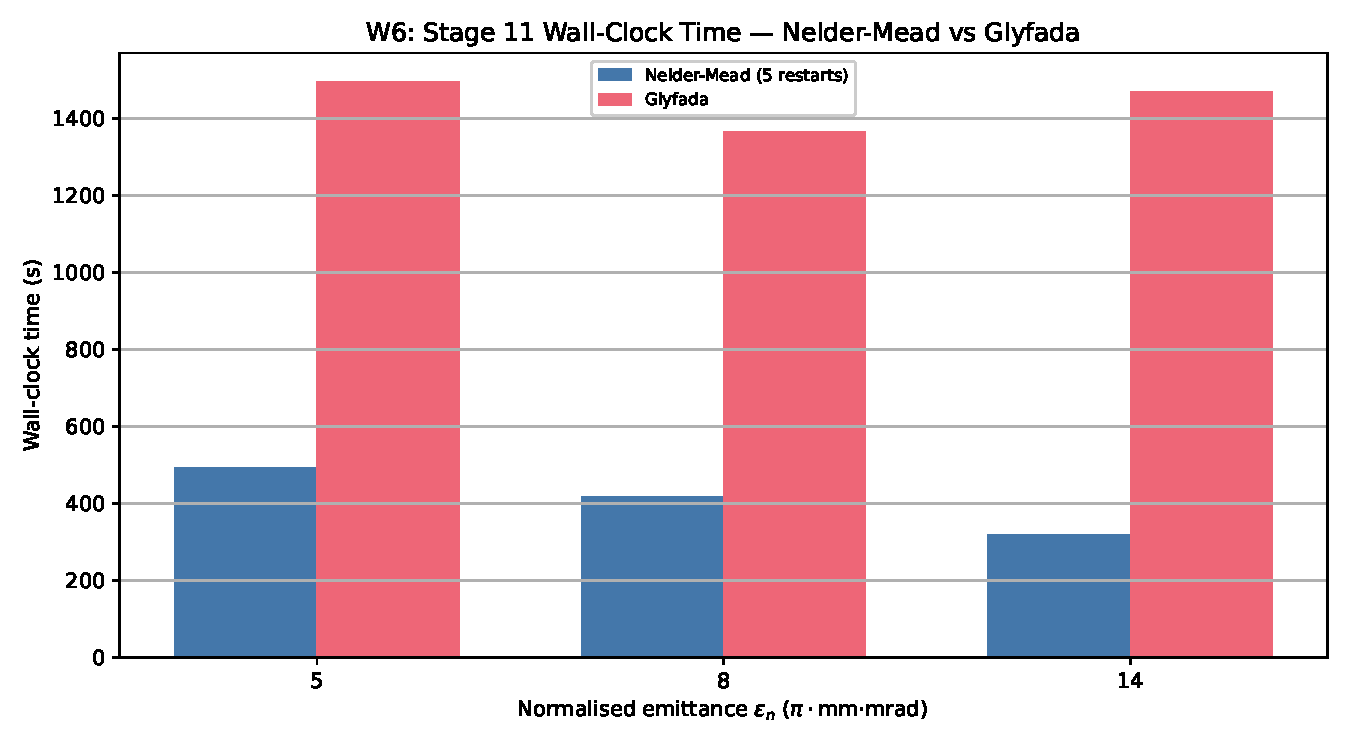
\includegraphics[width=0.85\textwidth]{results/params_05ps/W6/time_comparison.pdf}
\caption{Wall-clock time comparison. Glyfada time includes both the
  Stage~1--10 NM optimization ($\approx$\SI{8}{min}) and the Stage~11
  evolutionary search.}
\label{fig:time}
\end{figure}


\section{Discussion}

\paragraph{Glyfada does not improve on NM.}
At all three emittance points, NM outperforms glyfada by 3--6 orders
of magnitude in MSE.  Glyfada's random population initialization
frequently samples parameter combinations that produce unstable beam
optics (NaN Twiss values), triggering the $10^6$ penalty.  The
$\varepsilon_n = 5$ landscape is particularly hostile: even 600
random samples fail to find a single stable point, while NM at least
reaches a local minimum (MSE $= 0.40$).

The poor performance is expected for three reasons:
\begin{enumerate}
  \item \textbf{Low evaluation budget.}  600 evaluations
    ($30 \times 20$) is insufficient for a 4D continuous
    search where large regions of the parameter space produce
    divergent optics.
  \item \textbf{No warm-starting.}  NM starts from a reasonable
    initial guess (the Stage~10 result), giving it a head start
    in the basin of attraction.  Glyfada samples uniformly over
    $[0, 15] \times [0, 10]^3$, wasting most evaluations in
    infeasible regions.
  \item \textbf{Penalty distortion.}  Mapping all infeasible points
    to $-10^6$ (glyfada's penalty for failed evaluations) creates
    a flat objective landscape that provides no gradient information
    to guide the evolutionary search.
\end{enumerate}

\paragraph{Subprocess overhead.}
The DH evaluator protocol spawns a new Python process for each
fitness evaluation.  With $\approx$\SI{2.5}{s} per evaluation and
600~total, each glyfada run takes $\approx$\SI{25}{min}.  NM runs
in-process and completes Stage~11 in 5--8~minutes (including 5
random restarts with 300--755 function evaluations).  The $3\times$
wall-clock overhead is dominated by the beamline simulation, not
subprocess spawning.

\paragraph{Path forward.}
An in-process global optimizer
(\texttt{scipy.optimize.differential\_evolution}) would:
(a) eliminate subprocess overhead,
(b) allow warm-starting from the NM initial guess,
(c) enable custom bounds informed by the Stage~10 solution, and
(d) support penalty-aware fitness shaping (e.g., constraint handling
via feasibility rules rather than large penalties).


\section{Summary}

\begin{enumerate}
  \item Glyfada's evolutionary search with the DH evaluator protocol
    does not improve on Nelder-Mead for Stage~11.  NM outperforms
    glyfada by 3--6 orders of magnitude in MSE at all tested
    emittance points.
  \item The primary bottleneck is not the optimizer algorithm but the
    evaluation protocol: uniform random initialization over wide
    bounds wastes most of the 600-evaluation budget in infeasible
    regions.  Warm-starting and tighter bounds (informed by
    Stage~10) are essential for this landscape.
  \item Wall-clock time is $\approx 3\times$ higher for glyfada
    ($\approx$\SI{25}{min} vs $\approx$\SI{7}{min} for NM with 5
    restarts), due to subprocess overhead and the larger evaluation
    count.
  \item The $\varepsilon_n = 5$ problem remains unsolved by both
    methods.
\end{enumerate}

\paragraph{Next steps.}
\begin{itemize}
  \item Add \texttt{scipy.optimize.differential\_evolution} as an
    in-process Stage~11 method with warm-starting from the NM
    initial guess and tighter bounds.
  \item Investigate the $\varepsilon_n = 5$ landscape (objective
    function cross-sections, basin structure).
  \item Consider constraint-handling strategies (feasibility rules,
    death penalty avoidance) for future evolutionary runs.
\end{itemize}


\begin{thebibliography}{9}
\bibitem{weinberg2025}
  M.~Weinberg, A.~Fisher, and R.~Li,
  ``Design of the UH Mark V Free Electron Laser,''
  arXiv:2510.14061v1, Table~I.
\end{thebibliography}

\end{document}
